\documentclass{article}
\usepackage{graphicx} % Required for inserting images
\usepackage{enumitem}
\usepackage{gensymb}
\usepackage[margin=1in]{geometry}
\title{Frames of Reference}
\date{}
\begin{document}

\maketitle

\section{Background}
An often overlooked point when discussing the world is distinguishing between objects themselves and their representation within some specific system. In philosophy, this was considered already in Ancient times (see Plato's Theory of Ideas). However, in mathematics and physics, this topic is also of great importance, yet it is rarely emphasized (I never really thought about it until starting university). As physics (and mathematics to some extent) is all about finding descriptions of and explanations to the real world, this distinction between the real world itself, and our description of it, is fundamental, and a natural first place to start when doing physics.
\\\\
\textit{Consider:} If I ask you, what is \textit{$\pi$}, and you answer $3.141592...$, many (annoying) mathematicians would rush to inform you (once again, annoyingly), that this is not $\pi$, because $\pi$ itself has an infinite number of non-recurring decimals, and so as you keep counting them up you will get close to $\pi$, but never quite get there. However, this misses an even more important reason why your endless rambling of decimals will \textit{never} be $\pi$, even if you continue until infinity. That is because the number $3.141592...$ is not $\pi$, but rather the \textit{representation} of $\pi$ within the decimal number system. In binary, the number would look completely different. And so,m $\pi$ as a concept (for instance, defined as the ratio of the cicrumference and diameter of the circle) exists \textit{outside} of whatever system you use to describe it. But the description itself will never be $\pi$.
\\\\
Ideally, as we go through these sessions, I would like for us to feel like we are discovering the physics we are doing on our own, as if we are the first to ever discover it. For this reason, as this is one of our very first sessions, I would like for you to imagine yourselves as a group of the very first physicists on Earth. You don't know yet that what you are is a physicist, and that what you are doing is physics (not even Jesus was a Christian). You have just observed some things in reality, and now you wish to describe them.

Ok, so Nepo and Savio have seen a lot of interesting things in their lives, and they have now gotten together and agreed that they would like to not just see, but \textit{observe}, and discuss what they see with each other, to hopefully find out something about the world. However, in their very first meeting, they run into a problem. Because they are still not super close friends, they have decided to stay at a 20 m distance from each other (a safe distance), and they are both not looking at each other, but looking at a 90 degree angle to each other. There is an apple sitting right in the middle between them. 

Nepo begins by saying: "That apple is 10 meters to the \textbf{right} of me". 

Savio says: "No, that apple is 10 meters to the \textbf{left} of me". 

Already there is disagreement! So, who is right, is the apple 10 meters \textbf{left} or \textbf{right} of me? Think about what causes the disagreement here.

For a modern person reading this (or in fact, probably even an ancient one), they will likely think that the disagreement is a bit silly and jump to try and sort it out between Nepo and Savio. The issue is that the "me"s in their two sentences are different, one refers to Nepo, and the other refers to Savio. For instance, if Nepo and Savio were instead to say:

"That apple is 10 meters to the \textbf{right} of Nepo".

and 

"That apple is 10 meters to the \textbf{left} of Savio". 

Suddenly, the disagreement is no longer there. Nepo can check that indeed, Savio is 20 meters to the right of him. So if the apple is 10 meters to the right of Nepo, then since Savio is another 20 meters along, the apple should be $10 - 20 = -10$ meters to the right of Savio (i.e. 10 meters to the left). A straightforward solution. So, what is the first lesson which Nepo and Savio have learnt here?

Namely, they have learnt (hopefully) that their individual observations of the world will not coincide (unless they are themselves in exactly the same position). As soon as they accept that all of their observations are \textbf{relative} to where they are themselves, then they find that there is agreement between each other, and the world \textit{makes sense}. When they changed the "me" to their individual names, they implicitly made conceded this, realizing that their observations of position of the apple was all relative to where they (either Nepo or Savio) were, and that the "me" was not a unified concept.

Now let's say that Nepo and Savio start from the same position, but Savio is moving with speed 1 m/s to the right. The apple is now sitting right at Nepo's feet. With what speed will Nepo see the apple moving? With what speed will Savio see the apple moving? What about if the apple is rolling with speed 1 m/s to the right?

When we move around in the real world, this fact is very obvious to us, which is why it is perhaps a bit unlikely that Nepo and Savio would actually disagree on this so furiously, because as humans we quickly realize that observations are relative to ourselves, and we learn to factor that in automatically to our descriptions. However, sometimes this aspect of \textit{relativity} still causes problems, for instance, think of standing on a big hill overlooking Kigali with a friend, and you wish to point to where your house is (your friend does not know the location). If you stand 5 meters apart, it is very difficult to give the right direction to your friend when pointing with your finger, because the direction will be significantly different for the two of you. Unlike the apple example, it is much harder to translate the direction from one person's perspective to the other. The solution? Move closer to each other.

The fact that we do this translation from one person's point of view to another's automatically in our day-to-day life means that it can actually be a bit difficult to wrap our heads around how important this is in physics. But we will see why now.

\subsection{Formalizing the discussion}
In physics (and mathematics), as soon as we wish to quantify observations made in space, we usually turn to a coordinate system. In mathematics, we are often working in some abstract space, so we don't really care about "where" in the world this coordinate system is based. In physics, really all we care about is reality itself, so where our coordinate system is placed in reality (is it centered around Kigali or Stockholm?) is really a very important question. And so, to "place" our coordinate system relative to the outside reality which we are actually trying to observe (note here the distinction between reality itself, which is fixed, and the coordinate system itself, which depends on our choices), we usually take some reference point. A coordinate system which is determined by some set of reference points, is called a \textit{frame of reference} or \textit{reference frame}. 

So, let's now consider what Nepo and Savio were doing, but a bit more formally. Essentially, what they both did was set up two separate reference frames. Let's replace the word "me" in their statements with "origin". This means that they have both picked coordinate systems with themselves at the origin. 

\textbf{Definition}: In physics, we always assume that an observer places themselves at the origin of their own reference frame (you are always the center of your own world).

Now, this means that all the measurements and calculations that they do will all be \textit{within} this reference frame. Once again, just to stress the point, the real world itself exists outside of this and will be the same regardless of what a physicist chooses to describe it. To decribe it, we must introduce a system of coordinates centered around some points. The price we pay for this is that all our calculations are all relative to this frame. 

Luckily, let's not despair at this seeming relativity! As long as we can translate between these different frames, then we can have a sensible discussion. For instance, considering how in math we can switch between the binary and decimal number system (once again, the numbers exist outside the number systems themselves). 

And even better than this, let's consider this from the olympiad context. Whenever there are many ways to do the same thing (in this case, many ways of representing reality), it means that there are tricks for us to use!

\subsection{So, how do you switch between reference frames?}
This is really the X million dollar question. When you're given a physics problem, it will typically be in some given reference frame (typically the lab frame). And so, how do you find what the system looks like in some other frame? This is left for you to figure out! Remember, physics has not been invented yet. A good place to start is how to translate between the coordinates in Nepo's and Savio's frame in the example where a) they are in different positions, and b) where they are moving with constant velocity relative to each other.

\subsection{For olympiads}
So far, we have learned some pretty fundamental truths about how to represent reality, particularly within physics. So what does all of this mean for the context of Olympiads? It means opportunity.

Anytime you are given a physics problem, that problem is some description of what is happening in \textit{reality} (you will very rarely be given a coordinate system to work with). It is then your choice as the olympiad problem solver to choose a way of representing this physical system in a way where you can reason about it. Hence, the reference frame is always your choice! As we have seen, there is no inherently "correct" reference frames, they are all just different choices of how to represent the same thing (reality itself is the only correct thing). This means that the very first thing you want to ask yourself is, how do I represent this system? Or specifically, what \textit{frame of reference} do I pick?

Oftentimes, this is by far the most significant choice you will make when solving a physics problem. Many problems are solved almost instantly by picking the right frame of reference, whereas in the wrong frame, they become extremely difficult (think about the case of trying to point to your house, either standing right by your friend or a few meters aways, the reference frame is important there).

So, how do you make this choice? As with most olympiad techniques, there is not a tried and tested formula which always works (that wwould make olympiads very easy). However, once again as withmost olympiad tehcniques, there are some (very) helpful general guidelines, which will typically give very good guidance on what reference frame to pick. The rest, is about practice!

Potentially useful frames are where:
\begin{itemize}
    \item some bodies are at rest
    \item some projections of velocities vanish
    \item motion is symmetric
\end{itemize}

\section{Check your understanding}
\begin{enumerate}

\item
A man runs to the front of a train at a velocity of 2.5 m/s relative to the train. If the train moves at a velocity of 12.0 m/s relative to the platform, calculate the velocity of the man relative to a static observer standing on the platform. Can you do it with the formalism we have developed for reference frames? What would we typically call this frame?

\item A ship moves along the equator to the east with velocity $v = 30$ km/hour. The southeastern wind blows at an angle $\varphi = 60\degree$ to the equator with velocity $v = 15$ km/hour. Find the wind velocity $v'$ relative to the ship and the angle $\varphi'$ between the equator and the wind direction in the reference frame fixed to the ship.

\item The traces of raindrops falling vertically on the window of a motor car moving at a velocity of $45$ km/h form an angle of $30\degree$ with the vertical. Determine their velocity.
\end{enumerate}

\section{Trying out the waters}
Some advice: the first question you want to ask yourself is, what is the right frame? Then, after you find yourself in the right frame, at some point many of these problems become geometric problems, where all you really want to consider is the vectors themselves (ignoring the physics that got you there in the first place). It can be useful to take a step back at that point, realize what type of problem it is that you are looking at, and go from "physics" mode to "math" mode. 
\begin{enumerate}

    \item The trajectories of two bodies moving with non-relativistic constant speeds are parallel in a particular inertial reference frame.
\begin{enumerate}
    \item Is it possible to choose another inertial frame of reference in which the two trajectories cross each other?
    \item If such a frame can be found, and the bodies are started with suitable initial conditions, then it could be arranged that they reach the crossing point at the same time. How can this be consistent with the parallel trajectories observed in the first frame of reference?
\end{enumerate}

    \item Two particles, 1 and 2, move with constant velocities $\mathbf{v_1}$ and $\mathbf{v_2}$. At the initial moment their radius vectors are equal to $\mathbf{r_1}$ and $\mathbf{r_2}$. How must these four vectors be interrelated for the particles to collide? (Think: what frame is good to consider this question in?)

    \item A cart is moving on a straight road with constant velocity $v$. A boy, standing in an adjoining meadow, spots the cart and hopes to get a ride on it. In which direction should he run to catch the cart? Solve the problem generally: denote the speed of the cart by $v$, the maximal speed of the boy by $u$, and take the initial positions of the cart and boy to be as shown in the figure.
\begin{figure}
    \centering
    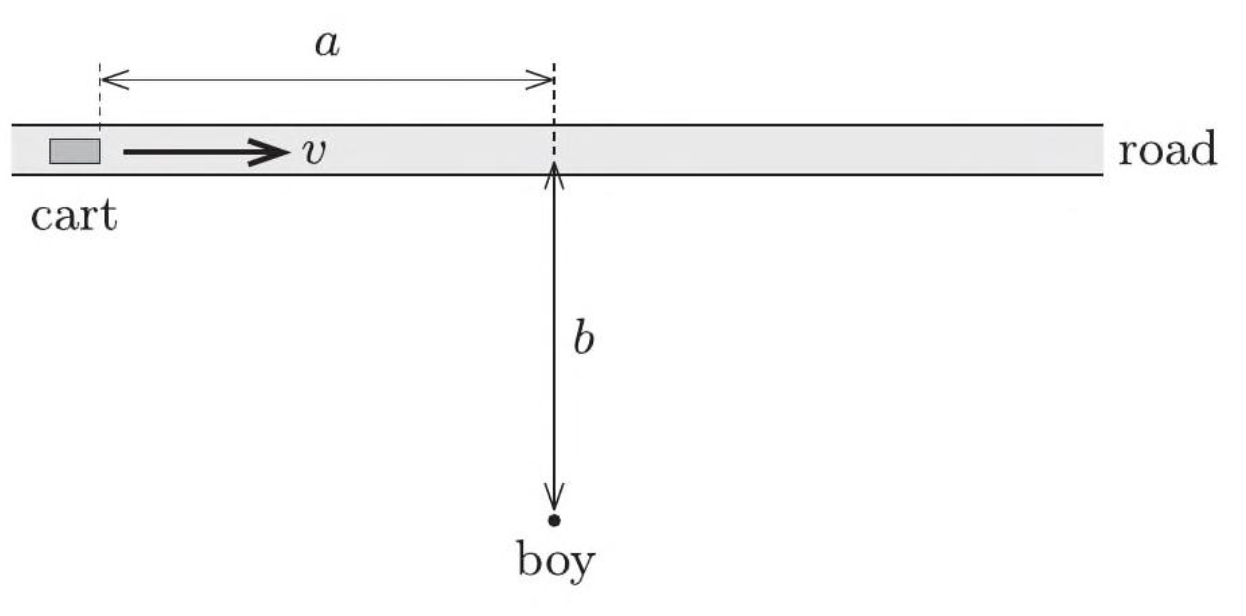
\includegraphics[width=0.5\linewidth]{cart and boy}
    \caption{Problem 3, cart and boy}
    \label{fig:enter-label}
\end{figure}
    \item A tube is mounted on a trolley which moves uniformly in a horizontal plane (see figure). At what angle to the horizontal should the tube be inclined so that a drop of rain, falling perpendicularly, should reach the bottom of the tube without touching its sides? The raindrop's rate of fall, $v_r$ is $60$ m/s (which does not alter, thanks to the effect of air-resistance). The speed of the trolley, $v_t$ is $20$ m/s.
    \item Two planes fly at the same height with speeds $v_1 = 800$ km/h and $v_2 = 600$ km/h, respectively. The planes approach each other; at a certain moment of time, the plane trajectories are perpendicular to each other and both planes are at the distance $a = 20$ km from the intersection points of their trajectories. Find the minimal distance between the planes during their flight assuming their velocities will remain constant.
    \begin{figure}
        \centering
        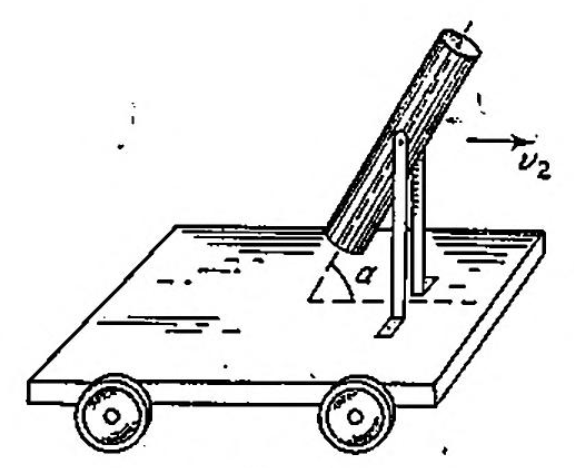
\includegraphics[width=0.5\linewidth]{trolley in rain}
        \caption{Problem 4, Trolley in rain}
        \label{fig:enter-label}
    \end{figure}
    \begin{figure}
        \centering
    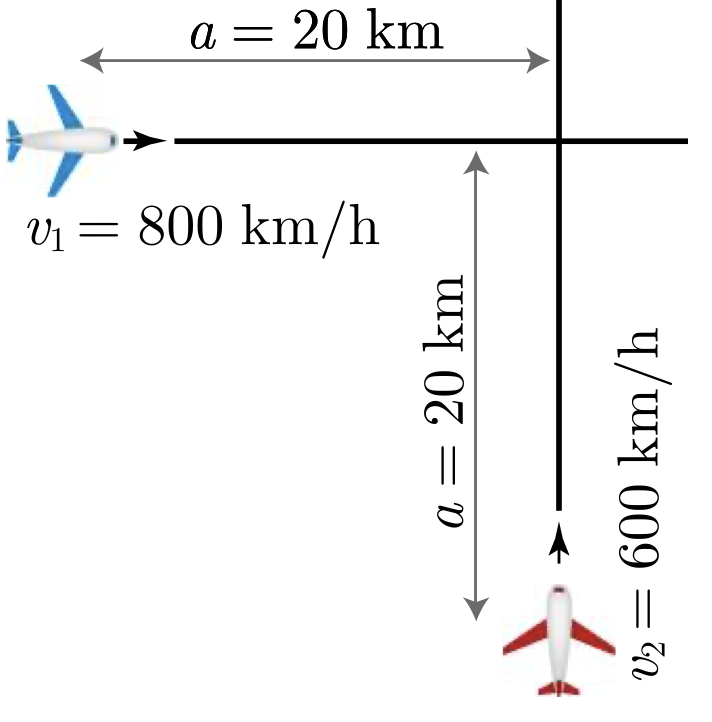
\includegraphics[width=0.5\linewidth]{Screenshot 2024-09-06 at 18.15.24.png}
    \caption{Problem 5, flying planes}
    \label{fig:enter-label}
\end{figure}

    \item A boat can travel at a speed of $3$ m/s on still water. A boatman wants to cross a river whilst covering the shortest possible distance. In what direction should he row with respect to the bank if the speed of the water is (i) 2 m/s, (ii), 4 m/s? Assume that the speed of the water is the same everywhere.

\end{enumerate}

\begin{enumerate}[resume]
    \item Two smooth slides lie within the same vertical plane and make angles $\alpha$ to the horizontal (see the figure). At some moment, two small balls are released from points A and B and they start sliding down. It took time $t_1$ for the first ball that started from point A to reach the ground; for the second one the time of descent was $t_2$. At what time was distance between the balls the smallest?
\end{enumerate}

\section{Explore the deep}
\begin{enumerate}
    \item One of two rings with radius $r$ is at rest and the other moves at velocity $\mathbf{v}$ towards the first one. Find how the velocity of the upper point of intersection depends on a, the distance between two rings’ centres.
\begin{figure}
    \centering
    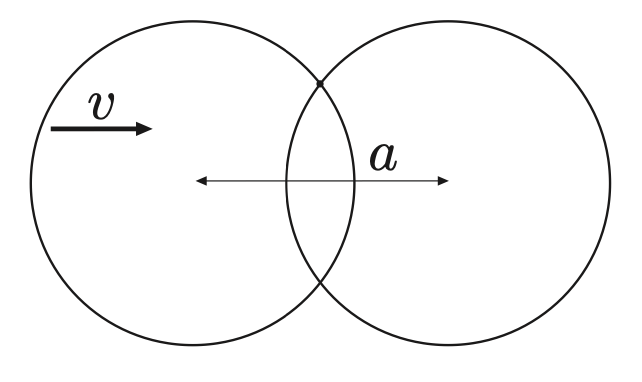
\includegraphics[width=0.5\linewidth]{Screenshot 2024-09-06 at 16.41.18.png}
    \caption{Problem 4.1, moving ring}
    \label{fig:enter-label}

\end{figure}
\end{enumerate}
\begin{enumerate}[resume]
    \item A tennis ball falls at velocity $v$ onto a heavy racket and bounces back elastically. What does the racket’s velocity $u$ have to be to make the ball bounce back at a right angle to its initial trajectory and not start spinning if it did not spin before the bounce? What is the angle $\beta$ between $\vec{u}$ and the normal of the racket’s plane, if the corresponding angle for $\vec{v}$ is $\alpha$?
    \item Three turtles are initially situated in the corners of an equilateral triangle at distances 1 m from one another. They move at constant velocity $v = 10$ cm/s in such a way that the first always heading towards the second, the second towards the third and the third towards the first. After what time will they meet?
\end{enumerate}
\section{Rwanda special question: Mzungu on moto}
Alice is driving with speed $v$ on a motorbike, and wishes to overtake a car right in front of her, of length $l$ and travelling with speed $u$. This will require her to enter the lane next to her, in which there is a car coming toward her in the opposite direction, also traveling with speed $u$ and currently a distance $L$ away, where $L > l$. You may ignore the length of the motorbike and the time it takes to switch lanes.

\begin{enumerate}[label=\alph*.]
\item What is the minimum speed $v_{min}$ with which Alice must travel in order to overtake the car in front of her without crashing into the car in the other lane?
\end{enumerate}

From now, we assume that $v \ge v_{min}$. In order to minimize the safety risk of overtaking the car in front, Alice would like to maximize the final distance $d$ between herself and the car in the other lane, when she switches back to her original lane after having taken over the car in front of her.

\begin{enumerate}[label=\alph*., resume]
\item Find the relationship between $d$ and the variables $v, u, L$, and $l$. Sketch $d$ as a function of $v$, for $v > u$. What is the optimal value of $v$ in order to maximize safety? Is it always better to have as high of a $v$ as possible?
\end{enumerate}

However, Alice realizes that while her \textit{actual} safety is maximized when $d$ is maximized, her \textit{perceived} safety is actually maximized when $T$ is maximized, where $t$ is the time passing between Alice switching back to her lane after overtaking the car in front and Alice passing by the car coming towards her in the opposite lane.  

\begin{enumerate}[label=\alph*., resume]
    \item Express $T$ in terms of $v, u, L$, and $l$, and sketch $T$ as a function of $v$. What is the optimal value of $v$ in order to maximize Alice's $perceived$ safety? You may assume that Alice continues to travel at speed $v$ after switching back to her original lane.
\end{enumerate}
\end{document}

